\subsection{Load Balancing}
Load Balancing ist eine wichtige Strategie, um die Leistung und Resilienz verteilter Systeme erheblich zu steigern. Hierfür wird die anstehende Arbeitslast dynamisch auf verfügbare Server oder Ressourcen aufgeteilt.

\subsubsection{Übersicht}
Drei Komponenten spielen hier eine wichtige Rolle. Im Mittelpunkt dieses Verfahrens steht der Load Balancer, eine Software- oder Hardwarekomponente, welche serverseitig über mehrere Dienste verwaltet. Die zweite Komponente ist eine Gruppe von gleichartigen Service-Instanzen, welche die eigentliche Geschäftslogik beinhalten. Eingehende Anfragen werden zuerst den Load Balancer gestellt, welcher diese dann mithilfe einer geeigneten Strategie möglichst gerecht auf die Service-Instanzen aufteilt.

Zuletzt ist eine Komponente von Nöten, welche verfolgt, wie viele Service-Instanzen in der Konstellation vorhanden sind und in welchem Zustand sich diese befinden, also Service Discovery bewerkstelligt. Dies erfolgt hier Server-Side: Ein Client hat keine Kenntnis über den Aufbau, also Topologie, dieses Systems \cite{schoner2017analyse}. Ob Load Balancing überhaupt Anwendung findet oder wie viele Ressourcen zur Verfügung stehen, wird nicht kommuniziert. Stattdessen geschieht jede externe Kommunikation nur mit dem Lastverteiler, welcher intern mithilfe der Registry ermittelt, welche Dienstknoten geeignet und bereit sind, die Anfrage entgegenzunehmen. Der Lastverteiler vermittelt nach Auswahl des Knotens schließlich zwischen dem Client und dem gewählten Service.

Load Balancing ist ebenso mit clientseitiger Service Discovery möglich. Hier existiert also kein zentraler Load Balancer, stattdessen ist der Client \textit{Registry-aware} \cite{schoner2017analyse} und wählt selbstständig einen passenden Serviceknoten aus, er verhält sich also selbst wie ein Load Balancer. Da die eigentliche Lastverteilungsmethodik dennoch ähnlich zur serverseitigen Discovery erfolgt und diese Methode speziell angepasste Clientsoftware benötigt, wird sie im weiteren Verlauf nicht näher erläutert.

\begin{figure}[t]
  \centering
  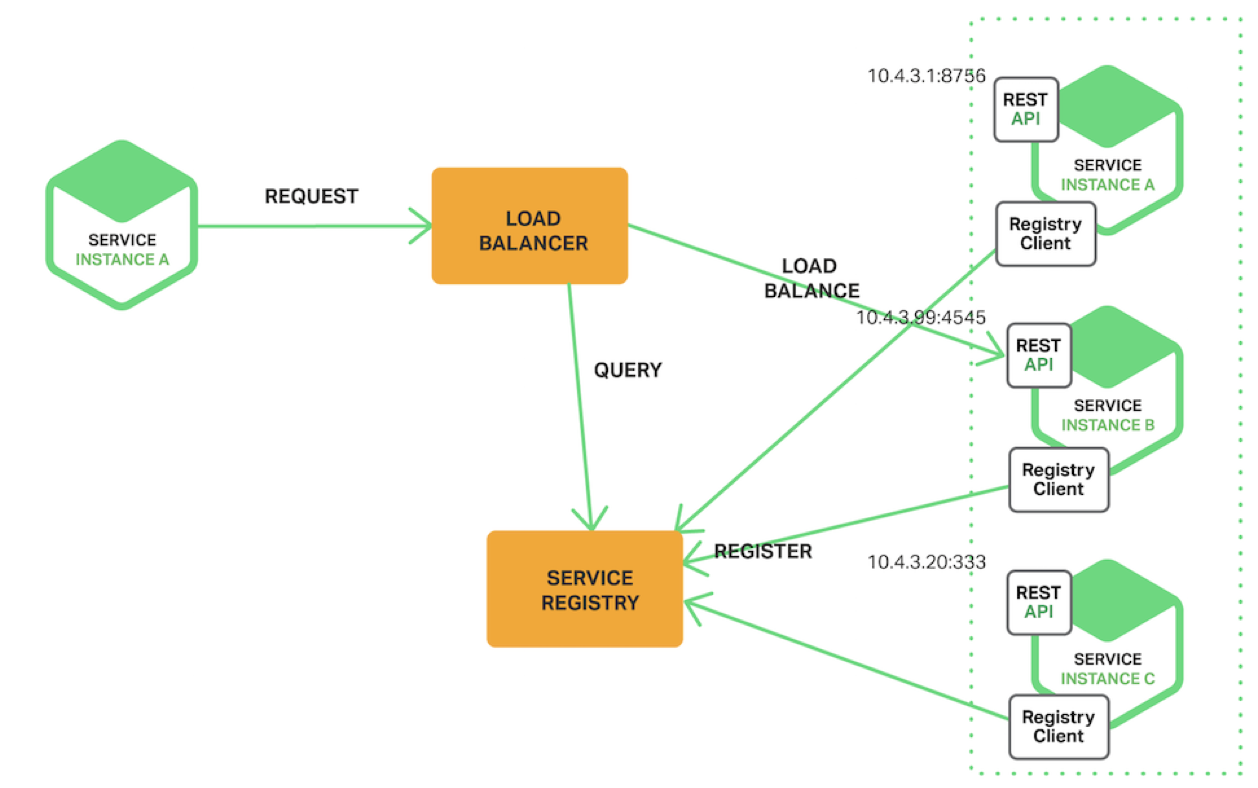
\includegraphics[width=\linewidth]{images/loadbalancer.png}
  \caption{Load Balancer mit drei Serviceinstanzen \cite{schoner2017analyse}}
    \label{fig:loadbalancer}
  \Description{Load Balancer mit Serverseitiger Service Discovery und drei Serviceinstanzen}
\end{figure}

In Abb.~\ref{fig:loadbalancer} werden die drei Komponenten mit dem typischen Datenfluss schematisch dargestellt: die Dienstinstanzen registrieren sich bei ihrem Start in der Service Registry. Erfolgt nun eine externe Anfrage an den Load Balancer, fragt dieser wiederum die Registry an, welche Dienste angemeldet sind. Mit dieser Information kann ein Dienst ausgewählt werden, und die eigentliche Anfrageverarbeitung kann stattfinden. Die Anfrage (Abb.~\ref{fig:loadbalancer}, links) erfolgt nie direkt an eine der Dienstinstanzen.
\subsubsection{Zustandsverfolgung der Dienste}
Im vorherigen Beispiel verfolgt die Service Registry zuerst nur, ob ein Service gestartet wurde. Dafür registriert bzw. deregistriert sich der Service zum Start bzw. planmäßigen Ende seiner Ausführung. Um eine effektive Lastverteilung zu ermöglichen reicht diese Information jedoch nicht aus. Wenn das Balancing ausschließlich realisiert wird, indem alle Anfragen \glq blind\grq{} auf Serviceknoten verteilt werden, könnten zwei Szenarien eintreten:
\begin{itemize}
	\item Obwohl die gleiche Anzahl an Anfragen fair an mehrere Knoten verteilt wird, könnte ein Knoten überlastet werden. Möglich wäre dies, wenn die entsprechenden Anfragen zufällig rechenintensiver sind als die Anfragen an andere Knoten. Ebenso denkbar ist, dass auf der Serverhardware andere Dienste oder (im Fall eines virtualisierten Computers) parallel ausgeführte virtuelle Maschinen mehr Rechenzeit verbrauchen (sogenannte \glqq Noisy Neighbours\grqq{}). Analog könnte eine langsamere Netzwerkanbindung zu unterschiedlichen Kapazitäten zwischen Knoten führen.
	\item Ein Serviceknoten könnte versagen. Beispielsweise könnte er ansprechbar sein, aber nur noch Fehlermeldungen zurückgeben. Alternativ antwortet er womöglich gar nicht mehr, oder benötigt derart viel Zeit, dass die Anfragen zum Zeitpunkt der Fertigstellung nicht mehr von Nutzen sind.
\end{itemize}

Es ist ersichtlich, dass ein pures Aufteilen der Anfragen auf 
%In beiden Fällen würde die Lastverteilung 

\subsubsection{Strategien der Lastverteilung}
Zu diesem Zeitpunkt 
Es ist bereits ersichtlich, dass hier alle drei Resilienzkategorien Anwendung finden: durch die Verwendung mehrerer 

Alle drei Hauptstrategien finden hier Anwendung: Durch mehrere verfügbare Ressourcen 